\documentclass{article}
\usepackage[utf8]{inputenc}
\usepackage[spanish]{babel}
\selectlanguage{spanish}
\usepackage{graphicx}

\title{Facultad de Ciencias \\Practica 1 \\ Fundamentos de Bases de Datos}
\author{Arteaga Hérnandez Alejandro Iabin \and Barocio Gómez Luis Fernando}

\date{Fecha de entrega: 19 Febrero 2020}

\begin{document}

\maketitle

\section{Manual de instalación}


\includegraphics[scale=0.5]{1}
\\
\textit{Para el primer paso de nuestra de PostgreSQL tenemos que agrega la GPG key, esta nos dará acceso a que podamos agregar el repositorio, comando es:\\ "wget --quiet -O - https://www.postgresql.org/media/keys/ACCC4CF8.asc | sudo apt-key add -"}


\includegraphics[scale=0.5]{2}
\\
\textit{Para el siguente paso es agregar el comando en la terminal para poder agregar el repositorio este comando es: \\ "sudo sh -c ’echo "deb http://apt.postgresql.org/pub/repos/apt/ DEB_VERSION-pgdg main" >> /etc/apt/sources.list.d/pgdg.list"}


\includegraphics[scale=0.5]{3}
\\
\textit{Ya casi para finalizar la instalación vamos a actualizar nuestros repositorios (sudo apt-get update) para poder instalar la paquetería necesaria ejecutamos el siguente comando "sudo apt-get install postgresql postgresql-contrib pgadmin4" confirmasmos u esperamos a que acabe}

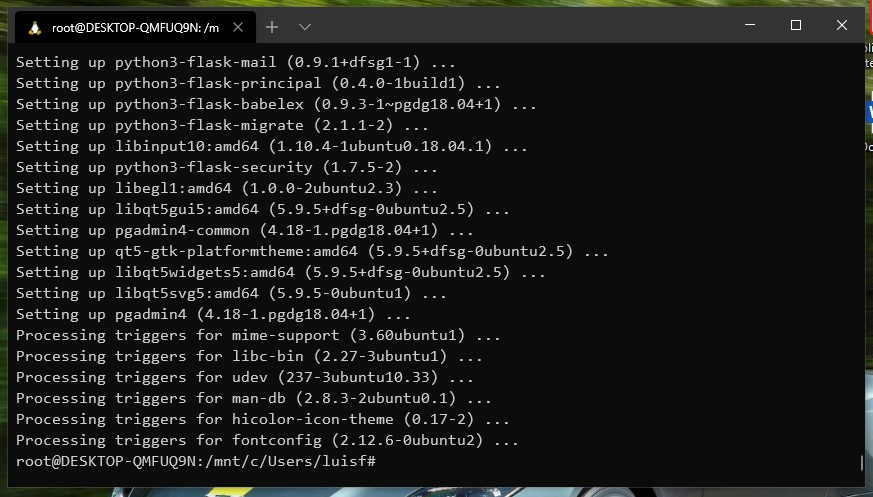
\includegraphics[scale=0.5]{4}
\textit{Finalmente tenemos que esperar hasta que nuestra terminal nos de linea de comandos nuevamente}

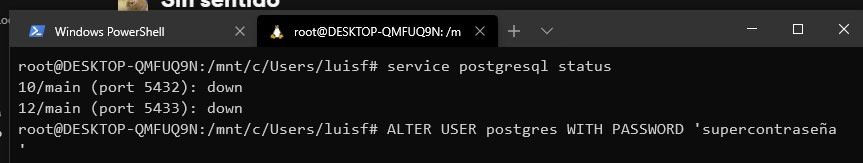
\includegraphics[scale=0.5]{5}
\texit{Para comprobar finalmente que fue instalado correctamente y un paso de seguridad vamos a correr este primer comando "service postgresql status" este nos muestra que esta "down" porque no lo hemos empezado.\\
finalmente solamente establecemos contraseña con el siguiente comando "ALTER USER postgres WITH PASSWORD ’my_password’;"}\\
\begin{itemize}
    \item Con esto tenemos por finalizada la instalación de PSQL en nuestro equipo, para cualquier paso de tener un fallo siempre es recomendable usar permisos de superusuario
\end{itemize}

\section{Preguntas}
\begin{enumerate}
    \item ¿Qué otros SMBD existen actualmente en el mercado? ¿Cuáles son las principales diferencias con PostgreSQL?
        \begin{itemize}
            \item MySQL: Es un sistema de gestión de base de datos relacional, multihilo y multiusuario seguramente el más usado en aplicaciones creadas como software libre.
    
            \item Las principales diferencias que se tienen entre ambos es que PostgreSQL es mucho mas "formal" se ocupa para proyectos mas grandes y en MySQL nos permite consultas mas rápidas un mayo compatibilidad con desarrollo web como puede ser PHP.
            
            \item PostgreSQL tiene un consumo de recursos mas alto que MySQL
            
            \item MySQL Es menos propenso a perdidas de datos en caso de fallar.
            
            \item PostgreSQL es capaz de tener mayor retro compatibilidad con versiones anteriores 
            
        \end{itemize}
    \item ¿Por qué una empresa debería escoger una base de datos open source?
    Las empresas por lo regular eligen bases de datos open source en el caso de querer ahorrar dinero, ya que el mantenimiento de estas y la renta de la base de datos les genera mas gasto, usando la base de datos open source solamente gastan en el manteamiento de esta. Otra razón puede ser el que sea una pequeña empresa y sus ingresos no sean tan elevados como para poder mantener una base de datos con licencia. 

    \item ¿Cuáles son las ventajas para un DBA escoger un SMBD open source?
    Una de las grandes ventajas es que al utilizar SMBD open source es que quien lo ocupa puede adaptarlo a sus necesidades ya que es código abierto 
    
    \item Describir a detalle qué es y para que sirve Docker y dar al menos 2 ejemplos de como podemos utilizar esta herramienta.
    
    \begin{itemize}
        \item Docker es uno de los proyectos más conocidos y utilizados en temas de virtualización esta plataforma de código abierto hace uso de las funciones de aislamiento de recursos del kernel de Linux para poder dar lugar a contenedores independientes, dentro de los cuales se ejecutará una única aplicación con sus respectivas dependencias, pero funcionando siempre con un único kernel, el de la máquina real, en lugar de virtualizar uno por cada contenedor o máquina virtual. Estos ejemplos pueden ser: 
        
        \item Simplificación de las configuraciones.

Una de las ventajas de la virtualización , es que podemos crear una máquina virtual, guardar el/los archivo/s y montarla en otro equipo manteniendo el último estado y la configuración en la parte superior de su estructura.
        
        \item Gestión de proyectos.

Uno de los mayores problemas a los que se enfrentan los equipos de desarrollo, es el tener que trabajar todos bajo el mismo entorno . Cada equipo sobre el que se va a poner a prueba la aplicación o servicio siempre tendrá algo diferente al resto, una actualización de menos (o de más), una librería de la que otros no dispongan, o directamente un sistema operativo u otro.
        
    \end{itemize}
    
    \item ¿Qué son las bases de datos No SQL? Menciona 3 ventajas y desventajas contra las bases relacionales.
    \begin{itemize}
        \item Ventajas Entre las principales motivaciones y características de las bases de datos NoSQL se
    encuentran: mayor simplicidad en el diseño, más facilidad para realizar escalamiento
    horizontal, mejor desempeño en aplicaciones en clústeres a gran escala. De hecho, estas
    bases de datos tuvieron una explosión en popularidad en la década de los 2000s debido a
    las necesidades de grandes empresas como Google, Microsoft, Amazon para alcanzar un
    mejor rendimiento en sus aplicaciones en la web.
    Como ya mencionamos, las bases de datos NoSQL no usan el modelo relacional en sus
    implementaciones. En su lugar, hay varios modelos de datos que se ocupan en este tipo de
    bases de datos en la actualidad, 
        
        \item Desventajas: A pesar de sus puestas en práctica en algunas grandes empresas, las bases de datos NoSQL aún se enfrentan a un problema de credibilidad importante con muchas empresas. Los críticos señalan la falta de madurez de NoSQL y los posibles problemas de inestabilidad, mientras que citan la madurez, y una gran funcionalidad y estabilidad de los RDBMSes. A diferencia de las bases de datos relacionales, que comparten ciertos estándares, las bases de datos NoSQL tienen pocas normas en común. Cada base de datos NoSQL tiene su propia API, las interfaces de consultas son únicas y tienen peculiaridades. Esta falta de normas significa que es imposible cambiar simplemente de un proveedor a otro, por si no quedara satisfecho con el servicio y la novedad de NoSQL significa que no hay una gran cantidad de desarrolladores y administradores que conocen la tecnología -lo que hace difícil a las empresas encontrar personas con los conocimientos técnicos apropiados. Por el contrario, el mundo RDBMS tiene miles de personas muy cualificadas ,algunas de ellas son:
        
        \item Documentales (MongoDB, CouchDB, Terrastore)
        
        \item Basadas en graficas (Neo4j, AllegroGraph, OrientDB)
        
        \item Llave/valor (Cassandra, BigTable, Dynamo)
        
        
    \end{itemize}
        
    
\end{enumerate}

\end{document}
